\documentclass[fleqn]{article}
\usepackage[english]{babel}
\usepackage{amsmath}
\usepackage{amsthm}
\usepackage{graphicx}
\usepackage[utf8]{inputenc}

%%%%%%%% MARGIN
\usepackage[left=1in, right=1in, top=0.8in, bottom=0.8in]{geometry}

%%%%%%%% NO PARAGRAPH INDENT
% https://tex.stackexchange.com/questions/27802/set-noindent-for-entire-file
\setlength\parindent{0pt}

%%%%%%%% SUB-FIGURE PACKAGE
\usepackage{subcaption}

\usepackage{pdfpages}

%%%%%%%% HYPERREF PACKAGE
\usepackage{hyperref}
\hypersetup{linkcolor=blue}
\hypersetup{citecolor=blue}
\hypersetup{urlcolor=blue}
\hypersetup{colorlinks=true}

%%%%%%%% MULTI-COLUMNS PACKAGE
\usepackage{multicol}

%%%%%%%% SETS DEFINITIONS
\usepackage{amssymb}
%%%% Important sets
\renewcommand{\O}{\mathbb{O}}
\newcommand{\N}{\mathbb{N}}
\newcommand{\Z}{{\mathbb{Z}}}
\newcommand{\Q}{{\mathbb{Q}}}
\newcommand{\RR}{{\mathbb{R}}}

%%%% Statistics
\newcommand{\E}[1]{\mathbb{E}\left[#1 \right]}
\newcommand{\V}[1]{\mathbb{V}\left[#1 \right]}
\newcommand{\cov}[1]{\mathrm{Cov}\left[#1 \right]}

%%% Misc Math
% Spaces after/before left/right
\let\originalleft\left
\let\originalright\right
\renewcommand{\left}{\mathopen{}\mathclose\bgroup\originalleft}
\renewcommand{\right}{\aftergroup\egroup\originalright}

% Norm and abs
\newcommand{\norm}[1]{\left\lVert#1\right\rVert}
\newcommand{\abs}[1]{\left\lvert#1\right\rvert}

%%%% Superscript to the left
% https://latex.org/forum/viewtopic.php?t=455
\usepackage{tensor}
\newcommand{\app}[3]{\tensor*[^{#1}]{\left(#2, #3\right)}{}}


%%%%%%%% SPLIT EQUATIONS
% https://tex.stackexchange.com/questions/51682/is-it-possible-to-pagebreak-aligned-equations
\allowdisplaybreaks

%%%%%%%% CODE RENDERING
% Compile with flag -shell-escape
\usepackage{minted}

%%%%%%%% EXAM PACKAGE
\usepackage{mathexam}

%%%%%%%% CHANGE MARGINS ITEMIZE
\usepackage{enumitem}

%%%%%%%% START DOCUMENT

\ExamClass{EC0301 - Time Series}
\ExamName{Assignment \#4}
\ExamHead{\today}

\let\ds\displaystyle

\begin{document}
 \vspace{0.3cm}
   % Information of the student
   \begin{itemize}[leftmargin=6.25cm, labelsep=0.5cm]

     \item[\textit{Name}] \scalebox{1.2}{David Plazas Escudero} % Name
     \item[\textit{Student code}] 201710005101 % Code

   \end{itemize}
\vspace{0.3cm}

% Each of the items to solve
\begin{enumerate}
\item \textit{Let $\{2,3,1,-1,-4,-2,0,2,1,-2\}$ be a sample of a given time series. Estimate $\hat{\rho}_1$, $\hat{\rho}_2$ and $\hat{\rho_3}$.}

The autocorrelations are estimated computationally with the formula
\begin{equation}
    \hat{\rho}_j=\dfrac{\hat{\gamma}_j}{\hat{\gamma}_0}
\end{equation}
where
\[
\hat{\gamma}_j=\dfrac{1}{n-1}\sum_{t=j+1}^n(x_t-\mu)(x_{t-j}-\mu).
\]
The code used to estimate the first three autocorrelations of the given series is presented below:

\begin{minted}{python}
import numpy as np

def autocov(x, j):
    s = 0
    mean = np.mean(x)
    n = np.size(x)
    for t in range(j, n):
        s += (x[t] - mean)*(x[t-j] - mean)
    return s/(n - 1)
    
def autocorr(x, j):
    return autocov(x, j)/autocov(x, 0)
    
x = [2, 3, 1, -1, -4, -2, 0, 2, 1, -2]
rs = []
for j in range(1, 4):
    rs.append(autocorr(x, j))
    print("rho_"+str(j), ":", autocorr(x, j))
\end{minted}
The obtained autocorrelations are $\hat{\rho}_1=0.4545$, $\hat{\rho}_2=-0.25$ and $\hat{\rho}_3=0.-0.59$.

\item \textit{Using the sample from last exercise, calculate $\hat{\rho}_1^1$, $\hat{\rho}_2^2$ and $\hat{\rho}_3^3$. Hint: Use the Yule-Walker equations to estimate the AR models.}
The code to calculate the partial autocorrelations is presented below:
\begin{minted}{python}
# returns vector of AR coefficients
def yule_walker(rs):
    j = rs.shape[0]
    A = np.ones((j, j))
    for k in range(j-1):
        A[(k+1):, k] = rs[:-(k+1), 0]
        A[k, (k+1):] = rs[:-(k+1), 0]
    return np.matmul(np.linalg.inv(A), rs)
    
# returns \hat{p}_j^j
def pacf(x, j, rs=None):
    if j == 1:
        return autocorr(x, j)
    else:
        if rs is None:
            rs = []
            for i in range(1, j+1):
                rs.append(autocorr(x, i))
            rs = np.reshape(rs, (len(rs), 1))

        return yule_walker(rs)[-1, 0]
        
for j in range(1, 4):
    print('rho_' + str(j) + str(j) + ':', pacf(x, j))
\end{minted}
and the estimated values are $\hat{\rho}_1^1=0.4545$, $\hat{\rho}_2^2=-0.5755$ and $\hat{\rho}_3^3=-0.2832$

\item \textit{Simulate the process $x_t=x_{t-1}+\epsilon_t-0.6\epsilon_{t-1}$. Take the first difference and make the plot for the standard and partial autocorrelation functions of this first difference. What can be concluded from these plots?}
Note that
\[
x_t=x_{t-1}+\epsilon_t-0.6\epsilon_{t-1} \implies x_t-x_{t-1}=\epsilon_t-0.6\epsilon_{t-1}\implies w_t=\epsilon_t-0.6\epsilon_{t-1}.
\]
Therefore, the first difference $w_t$ is an MA(1) process with parameter $\theta_1=0.6$. Therefore, the autocorrelation plot must show a single spike (besides the 0-lag spike) exactly in the first lag, and the remaining autocorrelations should be close to 0. Furthermore, according to what was explained in class, the partial autocorrelation plot for an MA($q$), particularly for $q=1$, must decrease exponentially.

The code to simulate the process and obtain the autocorrelation and partial autocorrelation plots is presented below:
\begin{minted}{python}
import scipy.stats as st
import matplotlib.pyplot as plt
import statsmodels.api as sm

plt.rc('text', usetex=True)
plt.rcParams.update({'font.size': 15})

def process(x0, T, theta, sigma2=1):
    e = st.norm.rvs(size=(T), loc=0, scale=sigma2**0.5)
    xs = np.zeros(T)
    xs[0] = x0
    for t in range(1, T):
        xs[t] = xs[t-1] + e[t] - theta*e[t-1]
    return xs

def diff(x):
    xs = np.zeros(x.size - 1)
    for t in range(xs.size):
        xs[t] = x[t+1] - x[t]
    return xs


xs = process(0, 10000, 0.6)
ws = diff(xs)

lags = 40
fig1 = sm.graphics.tsa.plot_acf(ws, lags=lags)
plt.xlabel("lag")
plt.ylabel("$\hat{\\rho}_j$")
plt.title("")
plt.savefig("acf.pdf", bbox_inches='tight')

fig2 = sm.graphics.tsa.plot_pacf(ws, lags=lags)
plt.xlabel("lag")
plt.ylabel("$\hat{\\rho}_j^j$")
plt.title("")
plt.savefig("pacf.pdf", bbox_inches='tight')
\end{minted}

The obtained plots for the autocorrelation and partial autocorrelation are presented in Figures \ref{fig:acf} and \ref{fig:pacf} respectively. Note that these plots confirm the situation above described for an MA(1) process.

\begin{figure}[H]
    \centering
    \begin{subfigure}[b]{0.45\textwidth}
        \centering
        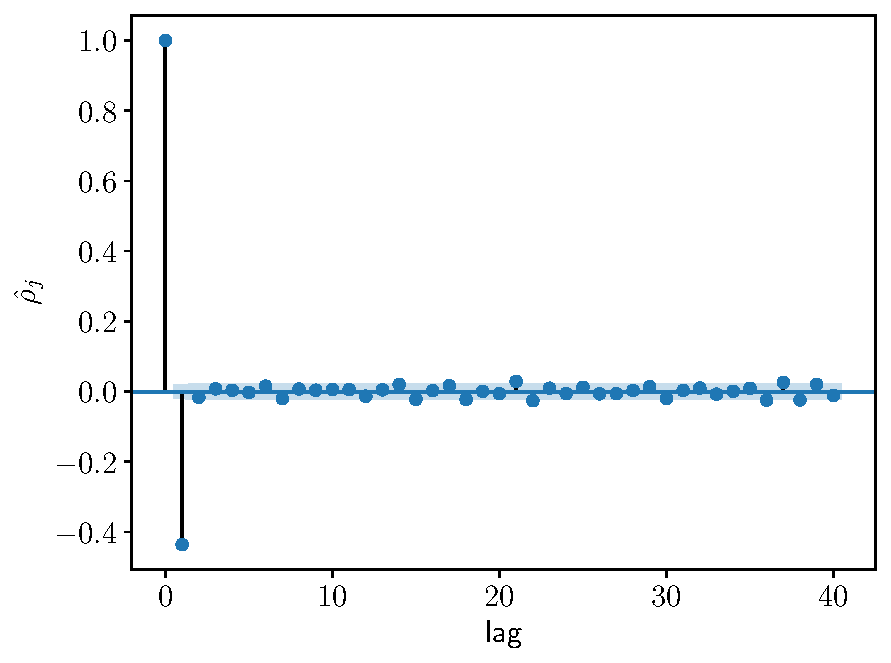
\includegraphics[width=\textwidth]{figs/acf.pdf}
        \caption{Autocorrelations.}
        \label{fig:acf}
    \end{subfigure}
    \begin{subfigure}[b]{0.45\textwidth}  
        \centering 
        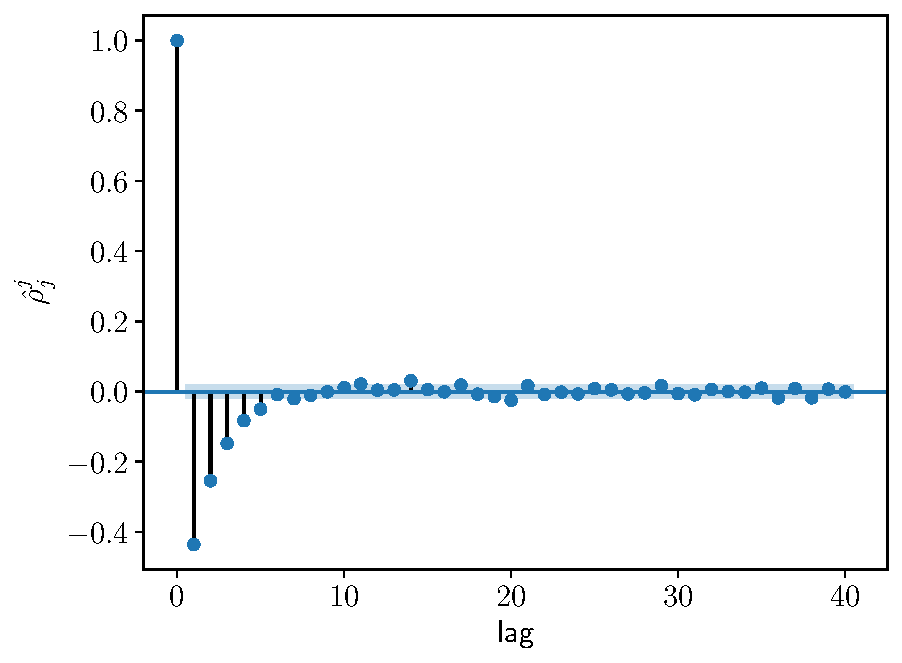
\includegraphics[width=\textwidth]{figs/pacf.pdf}
        \caption{Partial Autocorrelations.}
        \label{fig:pacf}
    \end{subfigure}
\end{figure}

\end{enumerate}
% \bibliographystyle{IEEEtran}
% \bibliography{bibs}
\end{document}
